\documentclass[tikz,border=8pt]{standalone}
\usetikzlibrary{arrows.meta}
\definecolor{bg}{HTML}{FBFBF9}
\definecolor{pred}{HTML}{DCEBFA}
\definecolor{prededge}{HTML}{2A6F97}
\definecolor{upd}{HTML}{E5F3E1}
\definecolor{updedge}{HTML}{2E7D4F}
\definecolor{meas}{HTML}{FDEBD3}
\definecolor{measedge}{HTML}{C9731B}
\definecolor{est}{HTML}{EEE5F7}
\definecolor{estedge}{HTML}{6A3FA0}
\definecolor{ink}{HTML}{233044}
\definecolor{sig}{HTML}{3A3F47}
\begin{document}
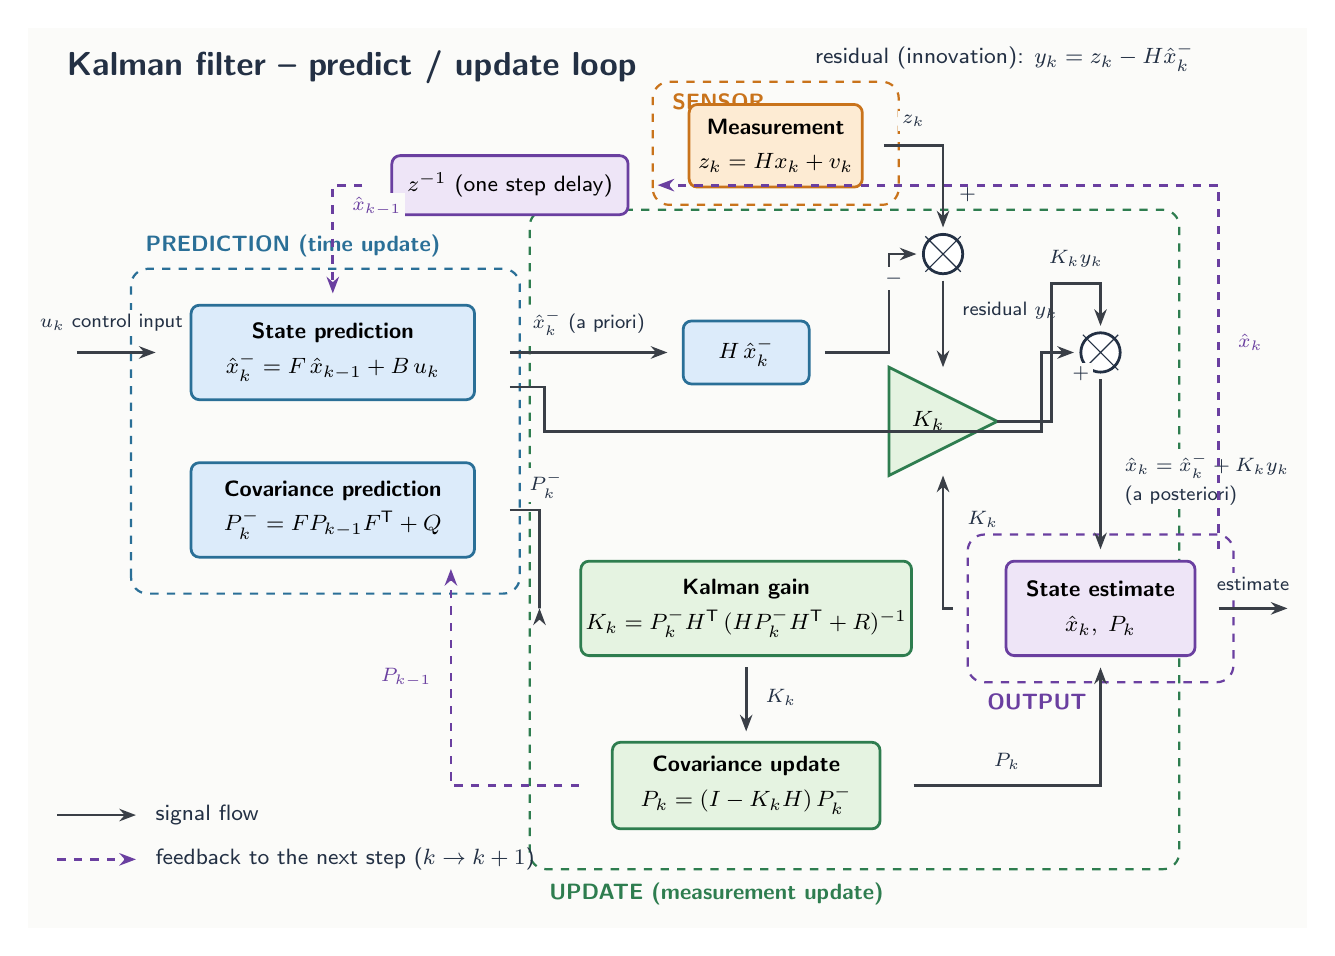
\begin{tikzpicture}[x=1.25cm,y=1.25cm,font=\sffamily\footnotesize,
  blk/.style={draw,line width=1pt,rounded corners=3pt,align=center,inner sep=0pt},
  sum/.style={circle,draw=ink,line width=1pt,minimum size=0.5cm,inner sep=0pt,fill=white},
  sigarrow/.style={-{Stealth[length=6pt]},line width=1pt,sig},
  fb/.style={-{Stealth[length=6pt]},line width=1pt,estedge,dashed},
  sl/.style={font=\sffamily\scriptsize,text=ink,fill=bg,inner sep=1.5pt},
  grp/.style={font=\sffamily\bfseries\footnotesize}]
  \fill[bg] (-0.7,-0.95) rectangle (12.3,8.2);
  \node[font=\sffamily\bfseries\large,text=ink,anchor=west] at (-0.4,7.8) {Kalman filter -- predict / update loop};

  % ===== group frames (drawn first) =====
  \draw[prededge,dashed,line width=0.8pt,rounded corners=6pt] (0.35,2.45) rectangle (4.3,5.75);
  \node[grp,text=prededge,anchor=west] at (0.4,5.98) {PREDICTION (time update)};
  \draw[updedge,dashed,line width=0.8pt,rounded corners=6pt] (4.4,-0.35) rectangle (11.0,6.35);
  \node[grp,text=updedge,anchor=west] at (4.5,-0.6) {UPDATE (measurement update)};
  \draw[measedge,dashed,line width=0.8pt,rounded corners=6pt] (5.65,6.4) rectangle (8.15,7.65);
  \node[grp,text=measedge,anchor=west] at (5.75,7.45) {SENSOR};
  \draw[estedge,dashed,line width=0.8pt,rounded corners=6pt] (8.85,1.55) rectangle (11.55,3.05);
  \node[grp,text=estedge,anchor=west] at (8.95,1.35) {OUTPUT};

  % ===== blocks =====
  \node[blk,draw=prededge,fill=pred,minimum width=3.6cm,minimum height=1.2cm] at (2.4,4.9) {\textbf{State prediction}\\[3pt]$\hat{x}^-_k = F\,\hat{x}_{k-1} + B\,u_k$};
  \node[blk,draw=prededge,fill=pred,minimum width=3.6cm,minimum height=1.2cm] at (2.4,3.3) {\textbf{Covariance prediction}\\[3pt]$P^-_k = F P_{k-1} F^{\mathsf T} + Q$};
  \node[blk,draw=measedge,fill=meas,minimum width=2.2cm,minimum height=1.05cm] at (6.9,7.0) {\textbf{Measurement}\\[3pt]$z_k = H x_k + v_k$};
  \node[blk,draw=prededge,fill=pred,minimum width=1.6cm,minimum height=0.8cm] at (6.6,4.9) {$H\,\hat{x}^-_k$};
  \node[blk,draw=updedge,fill=upd,minimum width=4.2cm,minimum height=1.2cm] at (6.6,2.3) {\textbf{Kalman gain}\\[3pt]$K_k = P^-_k H^{\mathsf T}\,(H P^-_k H^{\mathsf T} + R)^{-1}$};
  \node[blk,draw=updedge,fill=upd,minimum width=3.4cm,minimum height=1.1cm] at (6.6,0.5) {\textbf{Covariance update}\\[3pt]$P_k = (I - K_k H)\,P^-_k$};
  \node[blk,draw=estedge,fill=est,minimum width=2.4cm,minimum height=1.2cm] at (10.2,2.3) {\textbf{State estimate}\\[3pt]$\hat{x}_k,\;P_k$};
  \node[blk,draw=estedge,fill=est,minimum width=3.0cm,minimum height=0.75cm] at (4.2,6.6) {$z^{-1}$ (one step delay)};
  \filldraw[draw=updedge,fill=upd,line width=1pt] (8.05,4.75) -- (8.05,3.65) -- (9.15,4.2) -- cycle;
  \node at (8.45,4.2) {$K_k$};
  \node[sum] at (8.6,5.9) {}; \draw[ink,line width=0.4pt] (8.42,5.72) -- (8.78,6.08) (8.42,6.08) -- (8.78,5.72);
  \node[sum] at (10.2,4.9) {}; \draw[ink,line width=0.4pt] (10.02,4.72) -- (10.38,5.08) (10.02,5.08) -- (10.38,4.72);

  % ===== signal flow =====
  \draw[sigarrow] (-0.2,4.9) -- (0.6,4.9); \node[sl] at (0.15,5.2) {$u_k$ control input};
  \draw[sigarrow] (4.2,4.9) -- (5.8,4.9); \node[sl] at (5.0,5.2) {$\hat{x}^-_k$ (a priori)};
  \draw[sigarrow] (7.4,4.9) -- (8.05,4.9) -- (8.05,5.9) -- (8.33,5.9); \node[sl] at (8.1,5.65) {$-$};
  \draw[sigarrow] (8.0,7.0) -- (8.6,7.0) -- (8.6,6.17); \node[sl] at (8.3,7.25) {$z_k$}; \node[sl] at (8.85,6.5) {$+$};
  \draw[sigarrow] (8.6,5.63) -- (8.6,4.75); \node[sl,anchor=west] at (8.75,5.32) {residual $y_k$};
  \draw[sigarrow] (9.15,4.2) -- (9.7,4.2) -- (9.7,5.6) -- (10.2,5.6) -- (10.2,5.17); \node[sl] at (9.95,5.85) {$K_k y_k$};
  \draw[sigarrow] (4.2,4.55) -- (4.55,4.55) -- (4.55,4.1) -- (9.6,4.1) -- (9.6,4.9) -- (9.93,4.9); \node[sl] at (10.0,4.68) {$+$};
  \draw[sigarrow] (10.2,4.63) -- (10.2,2.9); \node[sl,anchor=west] at (10.4,3.75) {$\hat{x}_k = \hat{x}^-_k + K_k y_k$}; \node[sl,anchor=west] at (10.4,3.45) {(a posteriori)};
  \draw[sigarrow] (11.4,2.3) -- (12.1,2.3); \node[sl] at (11.75,2.55) {estimate};
  \draw[sigarrow] (4.2,3.3) -- (4.5,3.3) -- (4.5,2.3) -- (4.5,2.3); \node[sl,anchor=west] at (4.35,3.55) {$P^-_k$};
  \draw[sigarrow] (6.6,1.7) -- (6.6,1.05); \node[sl,anchor=west] at (6.75,1.4) {$K_k$};
  \draw[sigarrow] (8.7,2.3) -- (8.6,2.3) -- (8.6,3.65); \node[sl,anchor=west] at (8.8,3.2) {$K_k$};
  \draw[sigarrow] (8.3,0.5) -- (10.2,0.5) -- (10.2,1.7); \node[sl] at (9.25,0.75) {$P_k$};

  % ===== feedback (dashed purple) =====
  \draw[fb] (11.4,2.9) -- (11.4,6.6) -- (5.7,6.6); \node[sl,text=estedge,anchor=west] at (11.55,5.0) {$\hat{x}_k$};
  \draw[fb] (2.7,6.6) -- (2.4,6.6) -- (2.4,5.5); \node[sl,text=estedge,anchor=west] at (2.55,6.38) {$\hat{x}_{k-1}$};
  \draw[fb] (4.9,0.5) -- (3.6,0.5) -- (3.6,2.7); \node[sl,text=estedge,anchor=east] at (3.45,1.6) {$P_{k-1}$};

  % ===== legend =====
  \draw[sigarrow] (-0.4,0.2) -- (0.4,0.2); \node[anchor=west,text=ink] at (0.5,0.2) {signal flow};
  \draw[fb] (-0.4,-0.25) -- (0.4,-0.25); \node[anchor=west,text=ink] at (0.5,-0.25) {feedback to the next step ($k \to k+1$)};
  \node[anchor=west,text=ink] at (7.2,7.9) {residual (innovation): $y_k = z_k - H\hat{x}^-_k$};
\end{tikzpicture}
\end{document}
